\section{Multipleksery}

\subsection{Symbol multipleksera 4-bitowego}

\begin{figure}[h!]
    \centering
    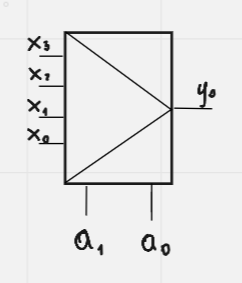
\includegraphics[width=0.35\textwidth]{images/mux/mux_s.png}
    \caption{Symbol multipleksera}
    \label{fig:my_label}
\end{figure}

Żeby odróżnić multiplekser od demultipleksera należy pamiętać, że MULTI-plekser ma MULTUM wejść. \textit{xd}
Podstawa trójkąta na ikonie jest ustawiona zawsze w stronę wejść. Zadaniem  multipleksera jest wybór za pomocą n wejść adresowych jednego z $2^n$ wejść danych. Multiplekser n-bitowy oznacza, że ma n wejść danych.

\subsection{Skrócona tabela prawdy}

\begin{figure}[h!]
    \centering
    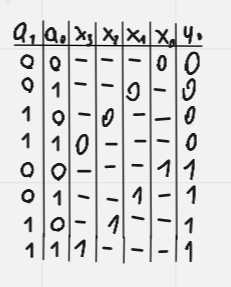
\includegraphics[width = 0.35\textwidth]{images/mux/mux_t.png}
    \caption{tabela prawdy dla multipleksera 4-bitowego}
    \label{fig:my_label}
\end{figure}

Nie ma sensu zapisywać całej tabeli prawdy, dlatego rozpisuje się jej uproszczoną wersję tak jak poniżej. Zgodnie z działaniem multipleksera nie ma sensu rozpatrywać wszystkich kombinacji, w końcu sygnały na wszystkich wejściach danych, poza wybranym przez wejścia adresowe, są pomijane.

\newpage

\subsection{Siatka karnaugh dla multipleksera 4-bitowego}

\begin{figure}[h!]
    \centering
    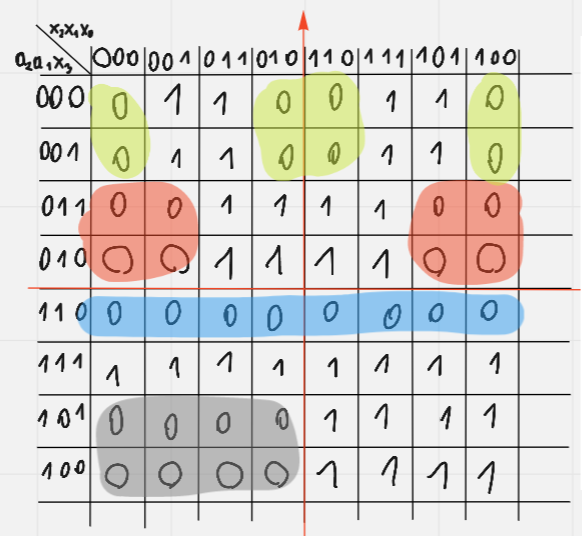
\includegraphics[width = 0.5\textwidth]{images/mux/mux_k.png}
    \caption{siatka karnaugha dla multipleksera 4-bitowego}
    \caption{siatka karnaugh}
    \label{fig:my_label}
\end{figure} 

Multiplekser był wykonywany w pełni na bramkach NOR więc w ramach ułatwienia, w siatce zaznaczane były implicenty (zera).

\subsection{Równie wynikowe}

\begin{figure}[h!]
    \centering
    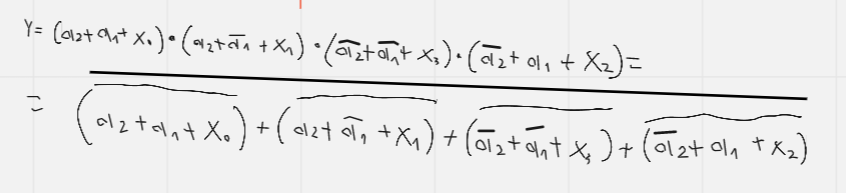
\includegraphics[width = 0.8\textwidth]{images/mux/mux_e.png}
    \caption{funkcja z siatki karnaugh}
    \label{fig:my_label}
\end{figure}

\newpage

\subsection{Schemat układu}

\begin{figure}[h!]
    \centering
    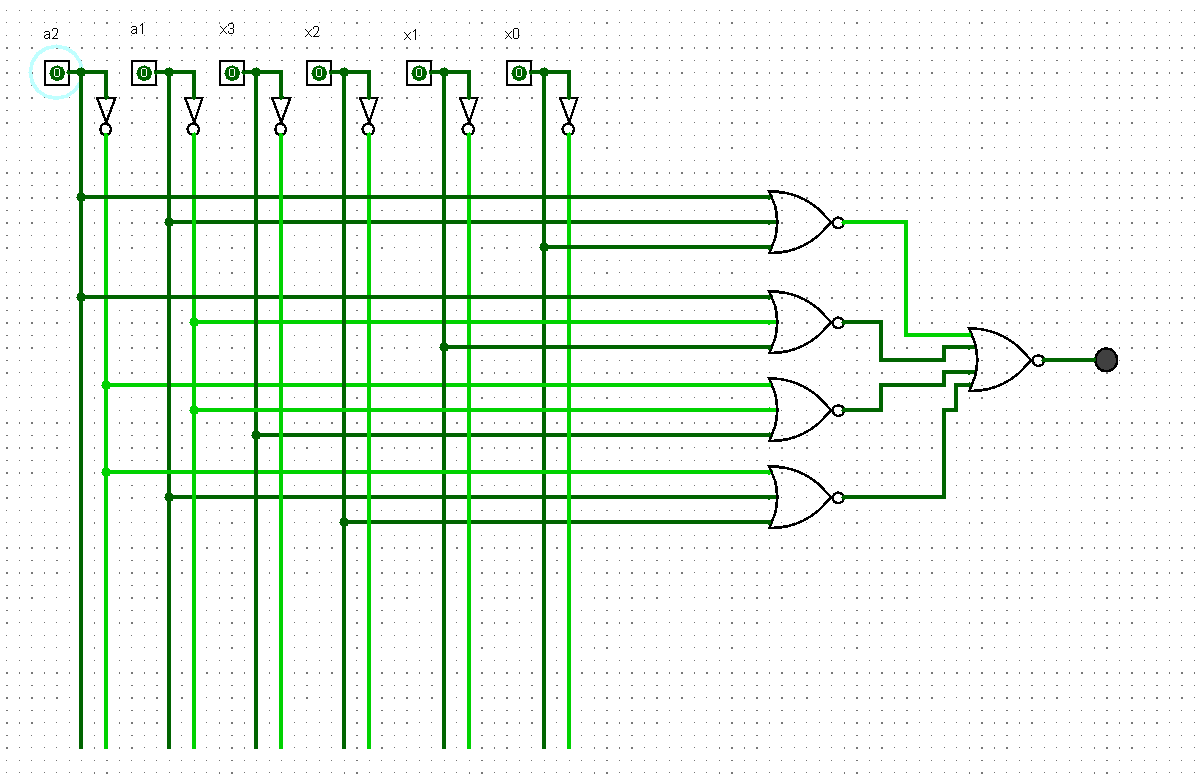
\includegraphics[width=\textwidth]{images/mux/mux_l.png}
    \caption{schemat układu}
    \label{fig:my_label}
\end{figure}

% e - równanie 
% k - karnaugh 
% t - tabelka
% s - schemat
% l - logisim
